\documentclass{article}
\usepackage{amssymb}% http://ctan.org/pkg/amssymb
\usepackage{pifont}% http://ctan.org/pkg/pifont
\newcommand{\cmark}{\ding{51}}%
% Updated definition, see explanation below
\newcommand*{\fullref}[1]{\hyperref[{#1}]{\autoref*{#1} \nameref*{#1}}} % One single link
\usepackage{geometry}
\usepackage{parskip}
\usepackage{pdflscape}
\usepackage{lscape}
\usepackage[colorlinks,pdfpagelabels,pdfstartview = FitH,bookmarksnumbered = true,linkcolor = black,citecolor = black]{hyperref}		% Inhaltsverzeichnis anklickbar
\usepackage{scrpage2} 									% Kopf- und Fusszeile
\pagestyle{scrheadings}
\renewcommand{\headfont}{\small}
\ihead{
\includegraphics[width=3cm]{NTB-FHO_LOGO}} % Kopfzeile links
\setlength{\headsep}{18mm}
\ohead{xl2DB}												 % Kopfzeile rechts
\ifoot{} 													 % Fusszeile links
\cfoot{\thepage}					 							     % Fusszeile mitte
\ofoot{}													 % Fusszeile rechts
\setheadsepline{0.4pt}										 % fügt horizontale linie ein 
\usepackage[utf8]{inputenc}
\usepackage[T1]{fontenc}
\usepackage{lmodern} % load a font with all the characters
\usepackage{graphicx}
\usepackage{caption}
\usepackage{subcaption}
\usepackage{enumitem}
\setlist[description]{leftmargin=\parindent,labelindent=\parindent}
\graphicspath{{Bilder/}}
\geometry{
	a4paper,
	total={210mm,297mm},
	left=25mm,
	right=25mm,
	top=28mm,
	bottom=25mm
}

\renewcommand{\contentsname}{Inhaltsverzeichnis}
\renewcommand{\listfigurename}{Abbildungsverzeichnis}
\renewcommand{\figurename}{Bild}

%%%%%%%%%%%%%%%%%%%%%%%%%%% BEGIN %%%%%%%%%%%%%%%%%%%%%%%%%%%%%%%%%%

\begin{document}
\begin{titlepage}


\pagenumbering{roman}

\title{Software Projekt - Excel als SQL Datenbank}
\author{Authoren: Rijad \v{Z}u\v{z}o, Séverin Müller \\ \\ Dozent: Ulrich Hauser}



\date{} 
\clearpage\maketitle
\thispagestyle{empty}

\vspace{80mm}
\begin{center}
		
\includegraphics[width=0.8 \textwidth]{SoftwareLogo}
\end{center}
\centering \huge "xl2DB"

\centering \normalsize Version: 0.9 vom 24.05.2015
\end{titlepage}
\newpage
\tableofcontents
\listoffigures
\newpage

\pagenumbering{arabic}

%%%%%%%%%%%%%%%%%%%%%%%%%%%  ERSTE SEITE  %%%%%%%%%%%%%%%%%%%%%%%%%%%

\section{Motivation}
Das Projekt wurde von uns in der Freizeit für den Bosnischen Club St. Gallen erarbeitet. Diese führen seit langem eine Excel-Liste für die Mitgliederverwaltung. \newline 
Für Sie war dies das einfachste Werkzeug, jedoch gab es immer wieder Probleme, wie zum Beispiel das ungewollte löschen ganzer Zeilen, oder das verrutschen in den Zeilen / Spalten. Wir wollten jedoch nicht eine komplett neue Datenbank erarbeiten, und entschieden uns, Ihnen ein Werkzeug für die Verwaltung der vorhandenen Excel Tabelle zur Verfügung zu stellen, welches eine einfache, intuitive GUI zur Verfügung stellt.

\subsection{Ausgangssituation}
Nebst den Problemen bei unaufmerksamer Bearbeitung, ist das Auslesen eines grösseren Excel Files deutlich langsamer als bei einer SQL Datenbank der gleichen bzw. einer vielfachen Grösse, deshalb ist es sinnvoll das Excel File in eine SQL Tabelle umzuwandeln und so zu Verarbeiten.

Die Konvertierung würde zusätzliche Software Kenntnisse erfordern, so griffen wir auf Vorhandene Office Werkzeuge bzw. vorhandene Excel Tabelle zurück.

Mit unserer x2dB Applikation wurde das Problem gelöst. Die Umwandlung ist dank ODBC Connector unnötig und somit kann das Excel File bestehend bleiben.

\subsection{Lösungsidee}
Wir legten vor allem Wert auf ein simples User-Interface mit allen nötigen Funktionen. Die Software verarbeitet das Excel File im Hintergrund als SQL Tabelle und verbindet sich mit entsprechenden Treibern über ein File das via GUI (Dateibrowser) eingebunden werden kann. Das ermöglichen uns die Microsoft.Office.Core\footnote{https://msdn.microsoft.com/en-us/library/microsoft.office.core.aspx}  und Microsoft.Office.Excel.Interop\footnote{https://msdn.microsoft.com/en-us/library/microsoft.office.interop.excel\%28v=office.15\%29.aspx} Treiber.

Mit unserer Applikation hat der User einen begrenzten Einfluss auf das File und kann so weniger Schaden am File anrichten. Schaden können auch gleichzeitige Lese- / Speicherzugriffe auf ein Shared File auf einem Netzwerklaufwerk. In unserer Applikation dauert die Verbindung nur kurz, bis die Daten gelesen/geschrieben wurden und danach wird das File wieder freigegeben. Parallele Bearbeitung ist in dieser Version nicht implementiert.

Für zusätzliche Datenintegrität wird jeweils ein Backup des Files erstellt und kann nötigen Falls zurück gespielt werden. Dies ist nicht die 'ultimative Lösung', aber wir konnten so die Sicherheit bei Veränderungen am Excel File erhöhen und trotzdem ein 'für jeden lesbares' Dateiformat weiter verwenden; dass zum Beispiel auch mit einem USB Stick übertragen und auf heimischen Computern (weiter-)bearbeitet werden kann.

\newpage

%%%%%%%%%%%%%%%%%%%%%%%%%%%  ZWEITE  SEITE  %%%%%%%%%%%%%%%%%%%%%%%%%%%

\section{Anforderungsliste}
Um die Bedürfnisse der Verwalter dieser Excel Liste bestmöglich abdecken zu können, haben wir uns mit Ihnen zusammengesetzt und die nachfolgenden Anforderungen definiert.
	
\subsection{Muss-Anforderungen}
Die Applikation muss:
	\begin{description}[labelindent=1cm]
		\item[M1:] das vorhandene Excel File als Datenbasis verwenden.
		\item[M2:] das Excel File lesen und beschreiben können.
		\item[M3:] nach dem Lesen bzw. Schreiben die Verbindung trennen.
		\item[M4:] bei Änderungen im File Backups erstellen.
		\item[M5:] dem User das Handling des Excel Files abnehmen.
	\end{description}

\subsection{Soll-Anforderung}
Die Applikation soll:
\begin{description}[labelindent=1cm]
	\item[S1:] leicht Bedienbar sein.
	\item[S2:] ein intuitives, einfaches User-Interface haben.
	\item[S3:] kompatibel mit Windows XP\footnote{http://windows.microsoft.com/de-de/windows/home} und höher sein.
	\item[S4:] kompatibel mit Excel 2003\footnote{http://www.office.com} und höher sein.
\end{description}

\subsection{Wunsch-Anforderung}
Die Applikation könnte:
\begin{description}[labelindent=1cm]
	\item[W1:] eine Benutzungsanleitung haben.
	\item[W2:] mehrere Sprachen unterstützen.
	\item[W3:] dem User Hilfe anbieten.
	\item[W4:] einträge sortieren.
	\item[W5:] auf Grund von Kriterien farbig hervorheben.
	\\
\end{description}

\vspace{2cm}

\textit{\textbf{Anmerkung}: Der Verein hatte noch einige Anforderungen an die Software, die rein vom Betriebssystem abhängig sind, deshalb wurden diese hier vernachlässigt.}
	

\newpage

%%%%%%%%%%%%%%%%%%%%%%%%%%%  DRITTE SEITE  %%%%%%%%%%%%%%%%%%%%%%%%%%%

\section{Projektumgebung}
\vspace{5mm}
\subsection{Entwicklungsprozess	}
Wir entschieden uns für den iterativen Scrum-Prozess\footnote{http://en.wikipedia.org/wiki/Scrum\_software\_development}. Es erschien uns Ideal, da wir jede Woche Dienstag mindestens zwei Lektionen Zeit hatten. Die Sprint Dauer passten wir aufgrund des Stundenplanes an (siehe: \nameref{sec:projektplanung}). Die Rollen teilten wir wie folgt auf:

\begin{description}
	\item[Scrum Master:] Rijad \v{Z}u\v{z}o
	\item[Management:] Séverin Müller
	\item[Product Owner \& Entwicklung] Rijad \v{Z}u\v{z}o, Séverin Müller
	\item[Customer] Verein
\end{description}

\subsection{Ablauf}
Die Stand-up Meetings erfolgten immer am Anfang der Lektionen am Dienstag bei einem Kaffee oder bei schönem Wetter kurz draussen. Wir benötigten jeweils kaum 10 Minuten, auch dank der guten Vorbereitung jeweils. Unter der Woche haben wir uns oft via Google Hangouts\footnote{https://google.com/hangouts} abgeglichen oder Fragen direkt mit der Freigabe eines Bildschirmes besprochen. 
Dank des Online-Tools Trello\footnote{http://www.trello.com/}  konnten wir die Aufgabenpakete sogleich zuteilen und die Meetings waren dank unserer Vorbereitung sehr speditiv. 

\subsection{Programmiersprache}
Da der Verein zuvor bereits Microsoft Excel verwendete und als Betriebssystem Microsoft Windows verwendete, lag es nahe, dass wir uns für die Windows Spezifische Programmiersprache C\# entschieden. \\ Dies in Kombination mit der IDE Visual Studio\footnote{https://www.visualstudio.com/} ermöglichte uns eine Praxis nahe und angenehme Entwicklung sowohl der Funktionalitäten,wie und auch des GUI's. 

\subsection{Verwaltungssystem}
Die Auswahl des Verwaltungssystem war sehr einfach, da wir uns im Vorhinein geeinigt haben die Software als OpenSource\footnote{http://de.wikipedia.org/wiki/Open\_Source} entwickeln zu wollen. Somit haben wir uns für das OpenSource Git Projekt Verwaltungssystem\footnote{http://git-scm.com/} entschieden und unser Code auf der Website www.GitHub.com gehostet.

Mit Hilfe dieser Collaboration Platform war es uns möglich, gleichzeitig, in unabhängigen Codeteilen, zu arbeiten und den jeweiligen Stand zu synchronisieren

\newpage

%%%%%%%%%%%%%%%%%%%%%%%%%%%  VIERTE SEITE  %%%%%%%%%%%%%%%%%%%%%%%%%%%

\section{Projekt Planung}
\label{sec:projektplanung}
	\begin{figure}[h]
		\subsection{Zeitplan}
		\bigskip
		\begin{center}
			\centering
			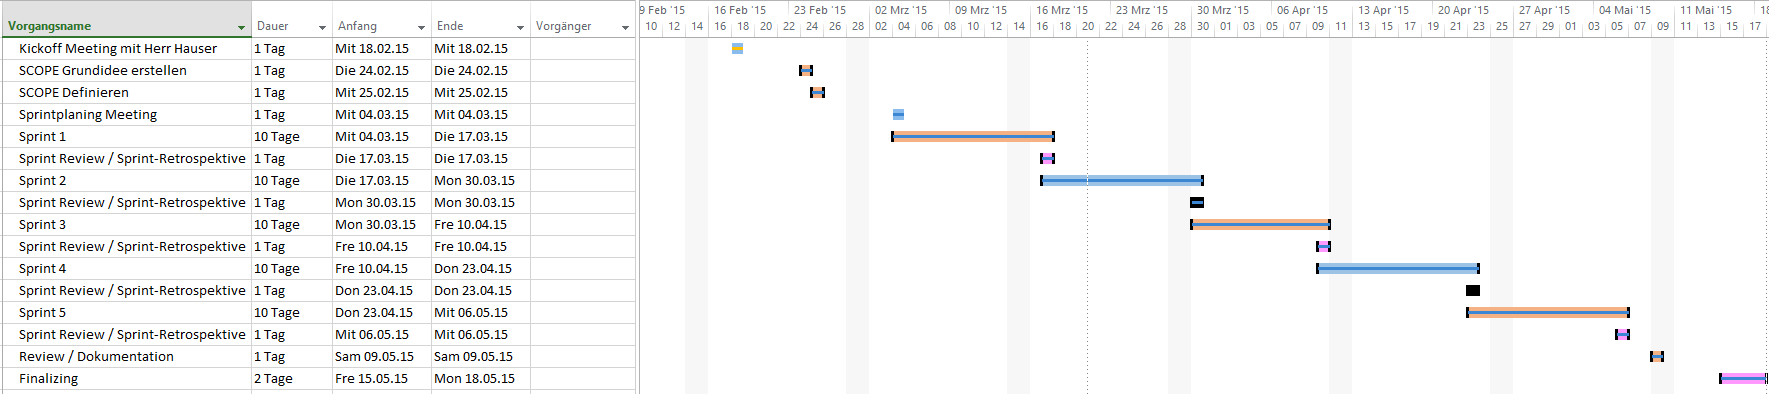
\includegraphics[width=0.8\paperwidth]{PJPlanung}
			\caption{Zeitplanung}
		\end{center}
	\end{figure}	
	
Wir haben uns auf eine Sprintdauer von 10 Tagen geeinigt. So hatten wir jeweils am Dienstag die Möglichkeit parallel weiter zu arbeiten und konnten Probleme oder offene Fragen klären. Die Sprints schlossen wir am Montag jeweils ab. Dies diskutierten wir entweder in der Waldau, St. Gallen am NTB oder kurz via Google Hangouts Videochat.

Das hat für uns sehr gut gepasst und die Atmosphäre sowie die Arbeiten waren angenehm. Die Sprintdauer war jeweils gerade richtig und der eingespielte Ablauf hat uns beiden sehr geholfen, wenn auch mal etwas dazwischen kam wie Prüfungen, Arbeit ... etc.
	
\subsection{Product Backlog}
\begin{figure}[h]
		\begin{center}
			\centering
			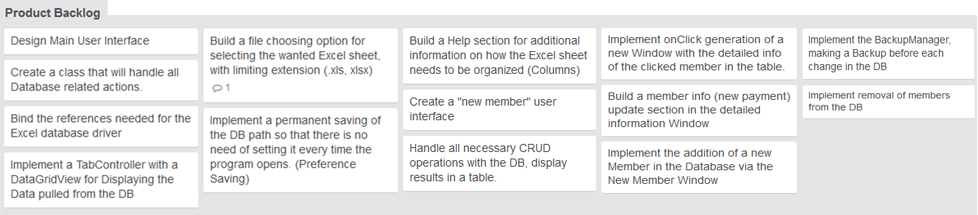
\includegraphics[width=0.8\paperwidth]{ProductBacklog1}
			\caption{Das Produkt Backlog}
		\end{center}
	\end{figure}
	
Wie schon erwähnt haben wir für die Planung der Applikation die Website Trello.com benutzt. Das Produkt Backlog ist im Bild 2 abgebildet.

Das grösste Problem Anfangs war die Aufteilung dieses Backlogs in sinnvolle und erreichbare Sprints. Dies haben wir dynamisch gelöst.

Wir haben einige Features zur Implementation ausgewählt und in einen Sprint mit entsprechender Deadline gepackt. Konnte ein Feature nicht in der gegebenen Zeit implementiert werden, wurde der Task in den nächsten Sprint mitgenommen oder zurück gestellt.

So sind wir auf fünf Sprints gekommen die in Bild 3. und Bild 4. dargestellt sind.

\newpage

%%%%%%%%%%%%%%%%%%%%%%%%%%%  FÜNFTE SEITE  %%%%%%%%%%%%%%%%%%%%%%%%%%%

\subsection{Sprints}
\begin{figure}[h]
	\centering 
	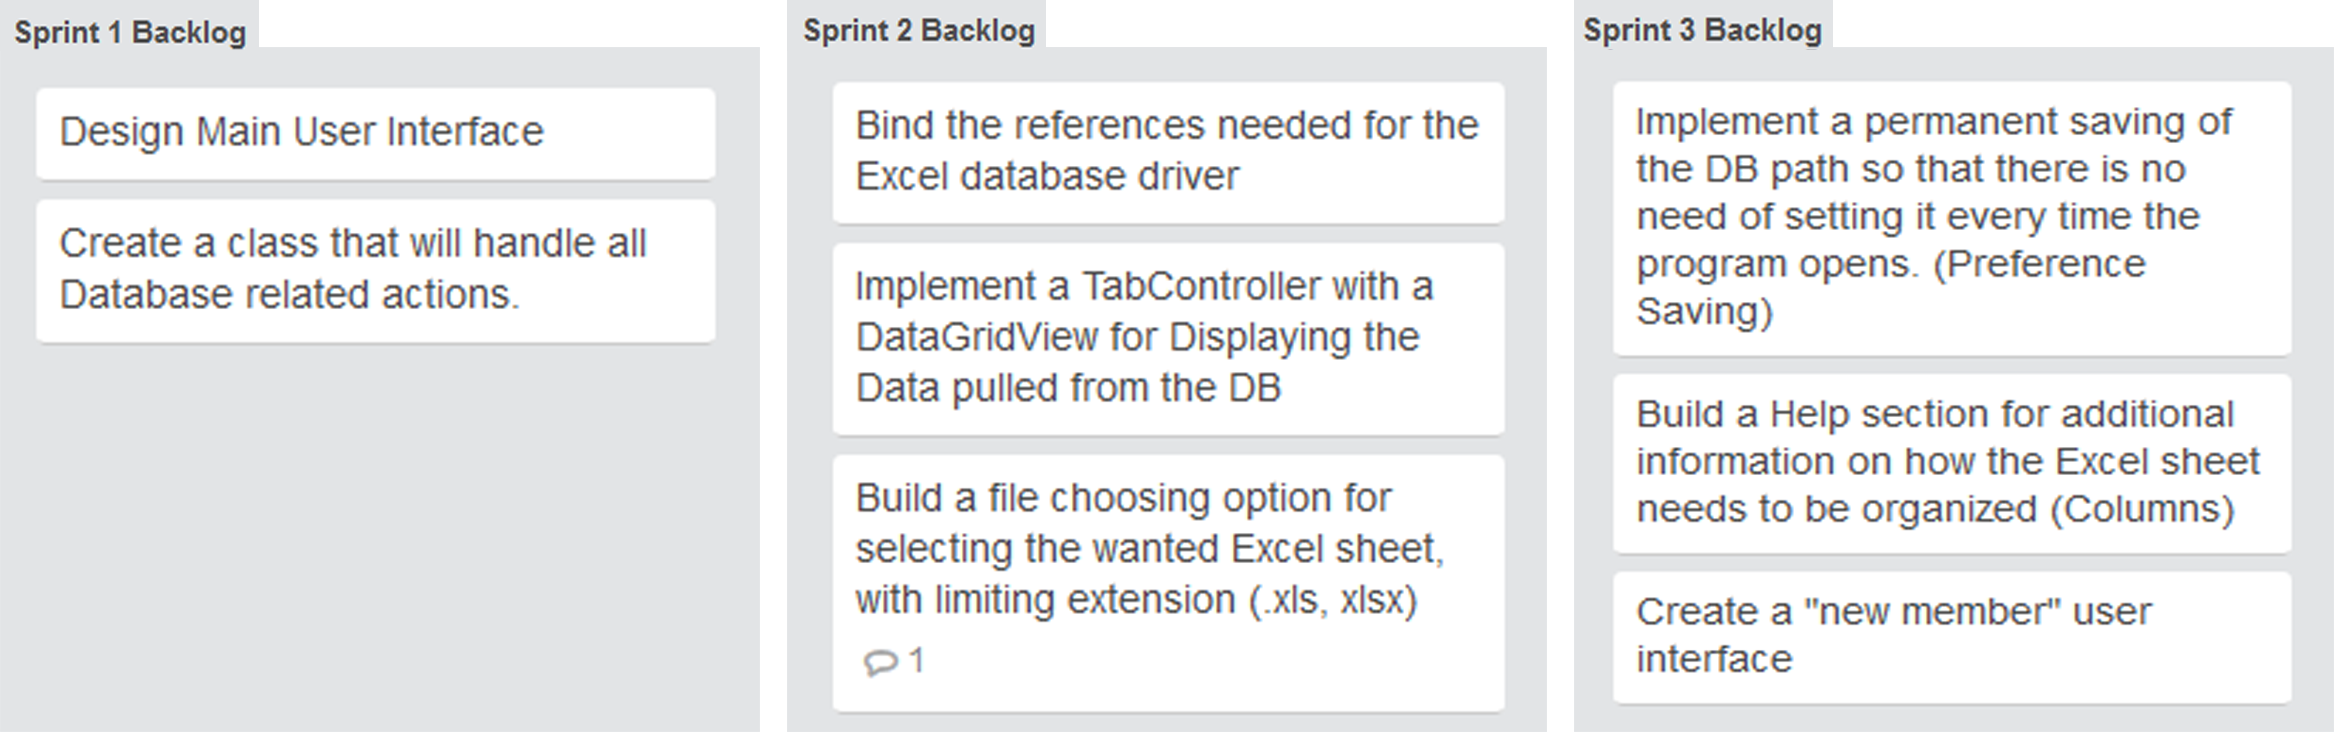
\includegraphics[width=0.6\paperwidth]{Sprint1-3}
	\caption{Sprints 1 - 3}
\end{figure}

\begin{figure}[h]
	\centering
	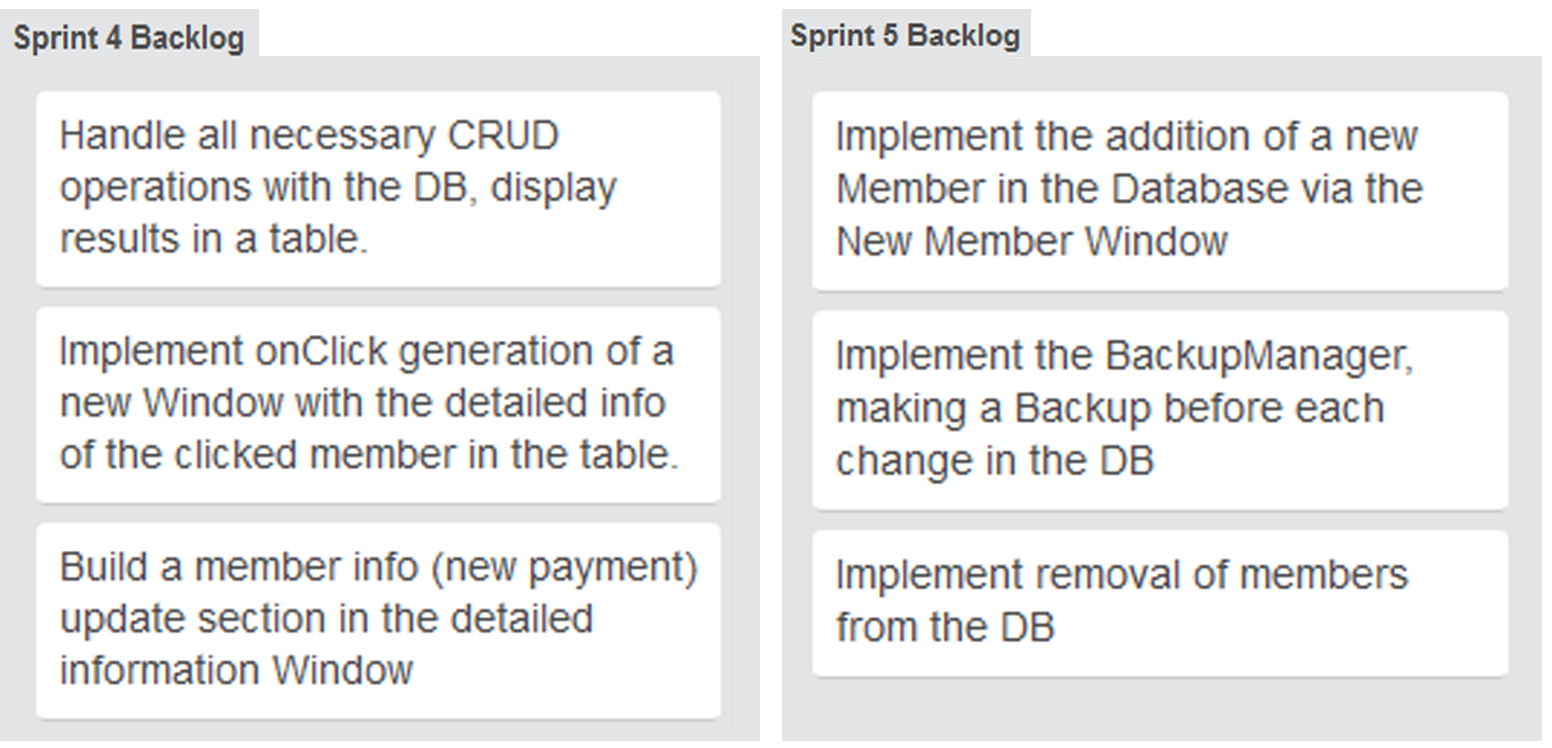
\includegraphics[width=0.4\paperwidth]{Sprint4-5}
	\caption{Sprints 4 - 5}
\end{figure}

\subsection{Sprint Stand-up Meetings}
Protokoll-artig auflisten was wir so besprochen haben usw.

\subsection{Sprint Review}
Review über all die Funktionalitäten und ob wir alles so erledigt haben wie es uns passt.

\newpage

%%%%%%%%%%%%%%%%%%%%%%%%%%%  SECHSTE SEITE  %%%%%%%%%%%%%%%%%%%%%%%%%%%

\section{Ablauf der Entwicklung}

\subsection{Modellierung}
Die erste Phase der Entwicklung war das Strukturieren der Software - eine sehr wichtige Phase. Wir wollten ein klares Design von Beginn an, dass uns die Weiterentwicklung ermöglicht.\\
Hier haben wir sehr viel Zeit aufgewendet, mit den Beteiligten sehr viele Szenarien durchgespielt und uns selbst einige Tage Zeit gelassen um über den Funktionsumfang und die Gimmicks eine klare Vorstellung zu erhalten. Die GUI sollte möglichst einfach gehalten sein, was aber nicht heisst, dass sich wenige Funktionen dahinter verbergen. 

\subsubsection{Klassendiagramm}
	
\begin{figure}[h]
	\centering
	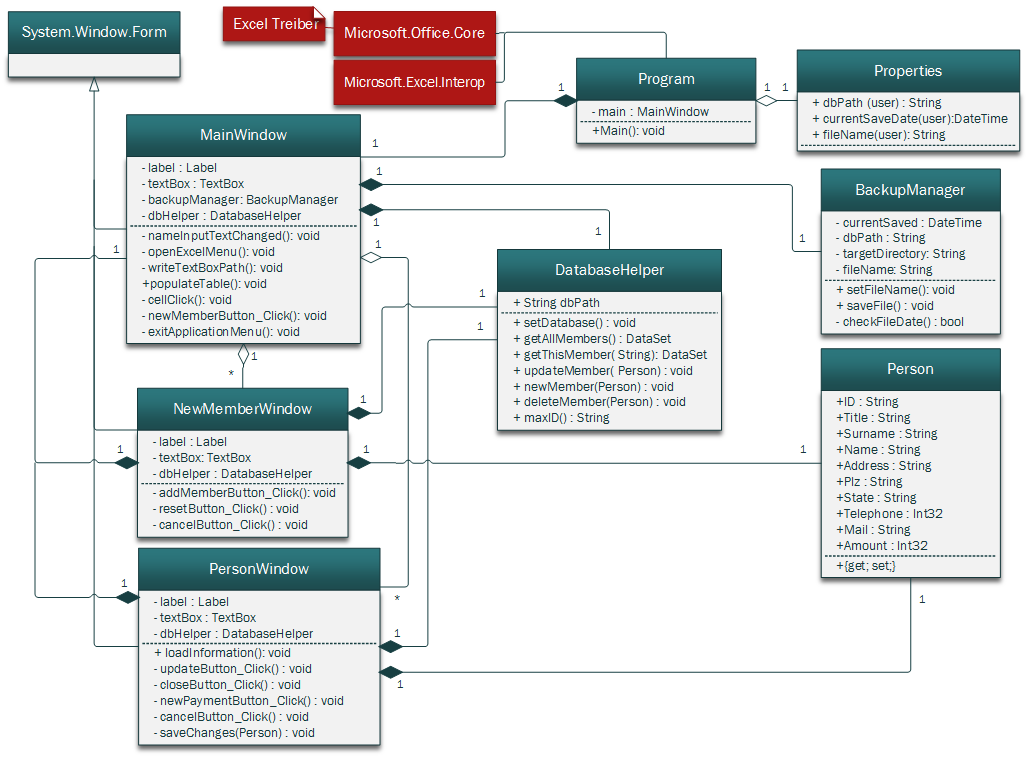
\includegraphics[width=1.05 \textwidth]{KlassendiagrammBild}
	\caption{Klassendiagramm}
\end{figure}

Eintritt in die Applikation geschieht durch die Main() Methode in der Klasse Program. Diese ruft den Konstruktor von MainWindow auf welcher die weitere Logik übernimmt. Im Microsoft Visual Studio 2013 werden die GUI Gestaltung und Logik automatisch getrennt, deshalb wurde im Klassendiagramm nur der Logische-Teil dargestellt.

Die MainWindow Klasse ist der Core der Applikation. Dieser nimmt die Eingaben vom User entgegen und leitet sie den entsprechenden Methoden und Klassen weiter. 

Die in Rot dargestellten Referenzen die den OleDB Treiber Beinhalten ermöglichen uns die Verbindung zu Excel Files. Das Excel File dient als Datenbank und kann mit diesen Treibern Ausgelesen und Beschreiben werden.

\newpage

%%%%%%%%%%%%%%%%%%%%%%%%%%%  SIEBTE SEITE  %%%%%%%%%%%%%%%%%%%%%%%%%%%

\subsubsection{Aktivitätsdiagramm}
\begin{figure}[h]
	\centering
	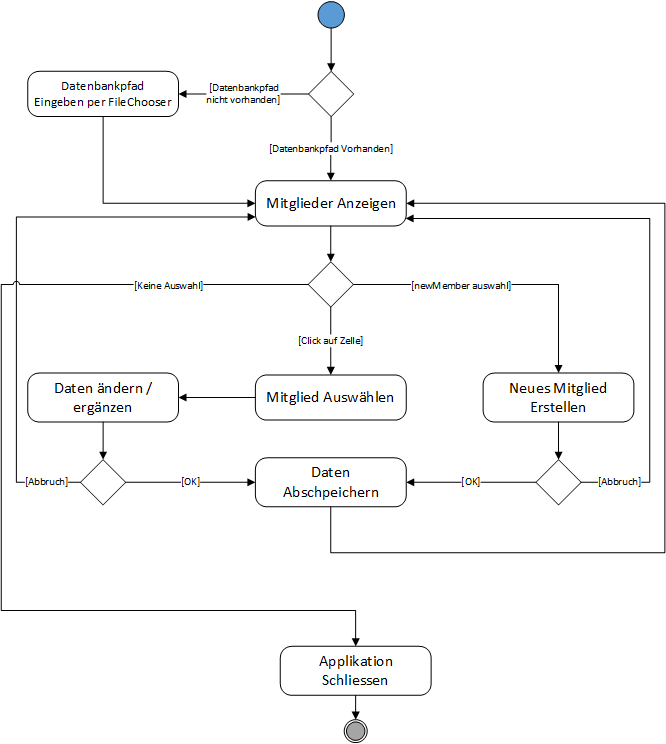
\includegraphics[width=0.9 \textwidth]{Aktivtaetsdiagramm}
	\caption{Aktivitätsdiagramm}
\end{figure}

Beim Start der Applikation wird überprüft ob bereits eine Datenbank hinterlegt ist oder nicht. Falls dieser vorhanden ist und verfügbar, werden alle Mitglieder automatisch aus der entsprechenden Datenbank ausgelesen und in der Tabelle dargestellt. Anderenfalls wird auf den User gewartet, bis dieser im File Chooser die gewünschte Datei (Datenbankpfad) manuell auswählt. 

Nach dem Auslesen der Mitglieder kann der User weitere Aktionen ausführen, wie z.B. ein neues Mitglied anlegen oder Mitglieder auswählen und detaillierte Informationen zur Person ansehen oder ändern.

Bei jeder Aktion kann der User seine Änderungen speichern oder alles verwerfen. Die Datenbank wird jeweils aktualisiert.

\newpage

%%%%%%%%%%%%%%%%%%%%%%%%%%%  NEUNTE SEITE  %%%%%%%%%%%%%%%%%%%%%%%%%%%

\subsubsection{Sequenzdiagramm}
\begin{figure}[h]
	\centering
	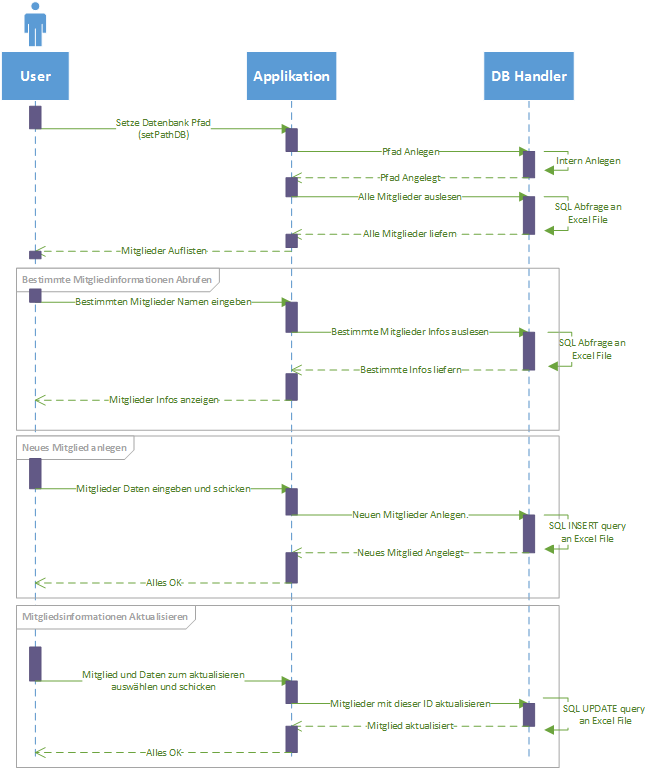
\includegraphics[width=0.8 \textwidth]{Sequenz-Diagramm_v1}
	\caption{Sequenzdiagramm}
\end{figure}

Setzt der User einen Datenbankpfad werden automatisch alle Mitglieder ausgelesen und angezeigt.
Im Sequenzdiagramm wurden mehrere Abläufe dargestellt: 
\begin{description}
	\item[Bestimmte Mitgliederinformationen Auslesen] \hfill \\ 
		Um nach einer Bestimmten Person zu suchen, gibt der User Name, Nachname, Adresse oder Ort ein. Jeder Tastenschlag setzt eine SQL Abfrage ab und entsprechende Datasets werden zurückgeliefert.
	
	\item[Neues Mitglied anlegen] \hfill \\  
		Falls der User ein neues Mitglied anlegen will, öffnet er das entsprechende Formular, gibt die neuen Daten ein und drückt den Save Button. Alle Daten werden in ein Datamodel gepackt und in der Datenbank angelegt.

	\item[Mitgliederinformationen Aktualisieren] \hfill \\ 
		 Falls der User ein Mitglied in der Liste anklickt, wird das Mitglied angezeigt. Hier kann er die Informationen aktualisieren oder das Mitglied löschen. Beim Löschen wird einfach ein "NULL update" gesendet, da das direkte Löschen im File nicht vom Treiber unterstützt wird.
\end{description}

\newpage

%%%%%%%%%%%%%%%%%%%%%%%%%%%  ZEHNTE SEITE  %%%%%%%%%%%%%%%%%%%%%%%%%%%

\subsection{GUI}
\subsubsection{Hauptfenster}
Die Oberfläche (GUI) wurde so einfach und intuitiv (selbsterklärend) wie möglich gestaltet. Dies auch auf Wunsche des Kunden:
\begin{figure}[h]
	\centering
	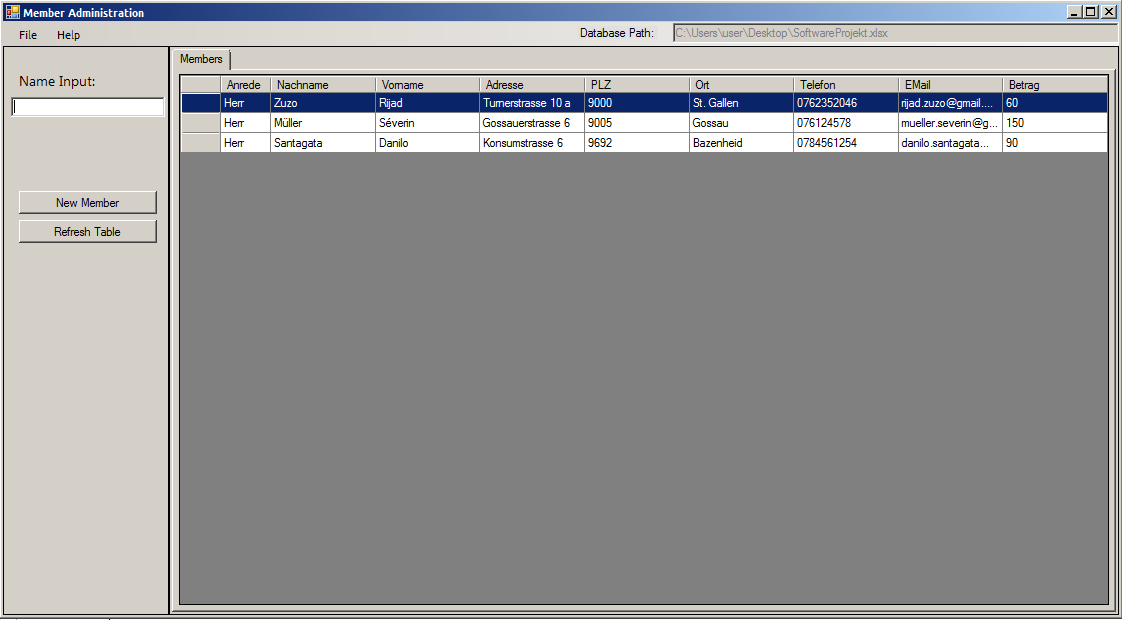
\includegraphics[width=1.0 \textwidth]{MainGUI}
	\caption{Hauptfenster}
\end{figure}

\begin{itemize}

		\item Das Excel File kann via FileChooser eingebunden werden
		\item Oben rechts wird der Pfad zur Datei "Database Path" angezeigt.
		\item Ein einfaches Texteingabe (text-input) Feld "Name Input" links, ermöglicht "on text change" (Eingaben werden sofort übergeben) die Suche nach: Nachname, Vorname, Adresse, Ort.
		\item Ein Klick auf ein Mitglied in der Tabellenansicht öffnet ein neues Fenster (Bild 9.b) und zeigt alle erfassten Details dessen.
		\item Unter Help gibt es eine einfache Anleitung "Excel Sheet Format Example" und ein Info Dialog mit Kontaktinformationen "About".
		\item Der Button "New Member" öffnet das Fenster (Bild 9.a) zum erstellen eines neuen Mitgliedes mit den nötigen Informationen.
		\item Der Button "Refresh Table" lädt das Excel File erneut. (Nützlich bei unerwartetem applikationsbenehmen)
	 \end{itemize}



\newpage

%%%%%%%%%%%%%%%%%%%%%%%%%%%  ELFTE SEITE  %%%%%%%%%%%%%%%%%%%%%%%%%%%

\subsubsection{Aufrufbare Fenster}
 \begin{figure}[h]
 	\centering
 	\begin{subfigure}{.4\textwidth}
 		\centering
 		\includegraphics[width=.5\linewidth]{NewMemberGui}
 		\caption{Neues Mitglied Formular}
 		\label{fig:sub1}
 	\end{subfigure}%
 	\begin{subfigure}{.5\textwidth}
 		\centering
 		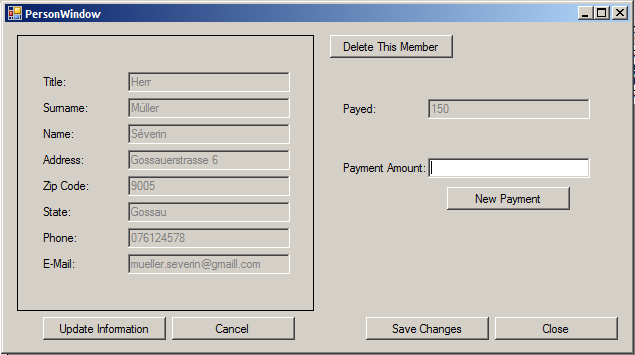
\includegraphics[width=.8\linewidth]{MemberInfoGUI}
 		\caption{Mitgliedsinformation Fenster}
 		\label{fig:sub2}
 	\end{subfigure}
 	\caption{Aufrufbare Fenster}
 	\label{fig:test}
 \end{figure}
 	\begin{itemize}
 	

	 \item Im Fenster "PersonWindow" (Bild 9.b) kann durch die Schaltfläche "Update Information" das Mitglied bearbeitet werden 				oder mit der Schaltfläche "Delete This Member" gelöscht werden.
 \item Ausserdem ist es Möglich den einbezahlten Mitgliederbeitrag (Payed) zu erhöhen (positver Betrag) oder ausstehende Beträge (negativer Betrag) ein zu pflegen (Payment Amount). Dies muss mit "New Payment" bestätigt werden.
 \item Ein Klick auf "Save Changes" speichert oder "Close" schliesst dieses Fenster ohne Speicherung.
 	\end{itemize} 


\vspace{10mm}
\textit{\textbf{Anmerkung}: Alle Änderungen werden sofort in das Excel File geschrieben. Es gibt keine zusätzlichen Abfragen! Änderungen werden jedoch beim Klick auf Close im jeweiligen Fenster verworfen.}

\subsection{Database Handling}
Wir haben die Klasse DatabaseHelper implementiert, in welcher alle Interaktion mit der Datenbank, in unserem Fall mit dem Excel File, stattfinden.

Aus den Referenzen Microsoft.Office.Core und Microsoft.Office.Excel.Interop haben wir den sogenannten OleDB Treiber nutzen können. Dieser hat uns das Auslesen und Beschreiben des Excel Files ermöglicht, jedoch unterstützt es keine direkte Löschen Operation. Dies haben wir umgangen, in dem wir das Excel File mit NULL Werten Beschreiben und solche Zeilen im GUI (in der Tabelle) ignorieren.

% Man kann das sicher besser formulieren
Um Zugriffskollisionen zu vermeiden, wird nach jeder Interaktion mit dem Excel File die Verbindung unterbrochen. Der Verbindungsmanager hält die Verbindung aufrecht, solange mit dem File gearbeitet wird (lesen/schreiben).
Das parallele bzw. gleichzeitige Bearbeiten des Excel Files ist in dieser Version noch nicht vollständig implementiert.

\subsection{Backup Management}
Wir unterstützen ein rudimentäres Backup des eingelesenen Excel Files. Die Datei wird bei der ersten Verwendung unter dem Pfad: \%username\%\textbackslash Desktop\textbackslash xlBackup gespeichert und umfasst jeweils eine Version beziehungsweise wird beim nächsten Aufruf überschrieben.

\textit{Anmerkung: Diese kann durch den Windows Schattenkopie Dienst (VSS) in weiteren Versionen geschützt werden.}

\subsection{Stunden Journal}

\section{Testen}
% Ab hier kopieren.
\textbf{GUI Tests\\}
\rule[2mm]{1\linewidth}{0.3mm}
\begin{tabular}{r|p{12cm}}
	1. Filechooser Test & Im Menu Strip -> File -> Choose Excel File \\
						& Ein File Chooser Menu wird aufgerufen. \hspace{5cm} \color{green} {\ding{51}} \\ \\
						
	2. Excel File Auswahl & Im File Chooser die gewünschte Datei auswählen und auf OK drücken. \\
							&	FileChooser wird geschlossen und die Tabelle mit Daten gefüllt \hspace{1.5cm} \color{green} {\ding{51}} \\
\end{tabular}
% Bis hier.
% Ab hier kopieren.
\textbf{GUI Tests Tests\\}
\rule[2mm]{1\linewidth}{0.3mm}
\begin{tabular}{r|p{12cm}}
	1. Filechooser Test & Im Menu Strip -> File -> Choose Excel File \\
						& Ein File Chooser Menu wird aufgerufen. \hspace{5cm} \color{green} {\ding{51}} \\ \\
						
	2. Excel File Auswahl & Im File Chooser die gewünschte Datei auswählen und auf OK drücken. \\
							&	FileChooser wird geschlossen und die Tabelle mit Daten gefüllt \hspace{1.5cm} \color{green} {\ding{51}} \\
\end{tabular}
% Bis hier.
% Ab hier kopieren.
\textbf{Failed Test\\}
\rule[2mm]{1\linewidth}{0.3mm}
\begin{tabular}{r|p{12cm}}
	1. Filechooser Test & Im Menu Strip -> File -> Choose Excel File \\
						& Ein File Chooser Menu wird aufgerufen. \hspace{5cm} \color{red}\ding{55} \\ \\
						
	2. Excel File Auswahl & Im File Chooser die gewünschte Datei auswählen und auf OK drücken. \\
							&	FileChooser wird geschlossen und die Tabelle mit Daten gefüllt \hspace{1.5cm} \color{red}\ding{55} \\
\end{tabular}
% Bis hier.
\newpage

%%%%%%%%%%%%%%%%%%%%%%%%%%%  ZWÖLFTE SEITE  %%%%%%%%%%%%%%%%%%%%%%%%%%%

\section{Ziel}
\subsection{Resultat}

Die Software "xl2DB" erfüllt die Muss- \& Soll-Anforderungen und erleichtert dem Verein das Handling der Mitglieder Datenbank nach ersten Rückmeldungen enorm. Dies ist für uns ein Erfolg. \\
Es sind noch Verbesserungen möglich, welche wir in Zukunft gerne noch einpflegen. Ausserdem sind die Wunsch-Anforderungen noch offen und bieten die Möglichkeit die Software noch attraktiver zu machen.

Wir haben in überschaubarer Zeit, erfolgreich eine Software entwickelt, die auch wirklich im Alltag eingesetzt werden kann. Der "Kunde" ist zufrieden und hat ein 'Wunsch' Werkzeug für sein Problem erhalten, dass ihn bei einem Individual-Softwarelieferanten ein ganzes Stück Geld gekostet hätte.

\subsection{Resultat: Muss-Anforderungen}
Die Applikation muss:
	\begin{description}
		\item[M1:] das vorhandene Excel File als Datenbasis verwenden. \color{green} {\ding{51}}
		\color{black}\item[M2:] das Excel File lesen und beschreiben können. \color{green} {\ding{51}}
		\color{black}\item[M3:] nach dem Lesen bzw. Schreiben die Verbindung trennen. \color{green} {\ding{51}}
		\color{black}\item[M4:] bei Änderungen im File Backups erstellen. \color{green} {\ding{51}}
		\color{black}\item[M5:] dem User das Handling des Excel Files abnehmen. \color{green} {\ding{51}}
	\end{description}
\vspace{5mm}
\textit{Es sind alle Muss-Anforderungen erfüllt.}

\subsection{Resultat: Soll-Anforderung}
Die Applikation soll:
\begin{description}
	\color{black}\item[S1:] leicht Bedienbar sein. \color{green} {\ding{51}}
	\color{black}\item[S2:] ein intuitives, einfaches User-Interface haben. \color{green} {\ding{51}}
	\color{black}\item[S3:] kompatibel mit Windows XP und höher sein. \color{green} {\ding{51}}
	\color{black}\item[S4:] kompatibel mit Excel 2003 und höher sein. \color{green} {\ding{51}}
\end{description}
\vspace{5mm}
\textit{Es sind alle Soll-Anforderungen erfüllt.}

\subsection{Resultat: Wunsch-Anforderung}
Die Applikation könnte:
\begin{description}
	\color{black}\item[W1:] eine Benutzungsanleitung haben. \color{green} {\ding{51}} \color{black}[rudimentär]
	\color{black}\item[W2:] mehrere Sprachen unterstützen.  \color{red}\ding{55}
	\color{black}\item[W3:] dem User Hilfe anbieten. \color{red}\ding{55}
	\color{black}\item[W4:] einträge sortieren. \color{red}\ding{55}
	\color{black}\item[W5:] auf Grund von Kriterien farbig hervorheben. \color{red}\ding{55}
\end{description}
\vspace{5mm}
\textit{Leider sind wir nicht dazu gekommen alle Wunsch-Anforderungen zu erfüllen. Hier gibt es Raum die Software weiter auszubauen und zu verbessern. Ein Projekt für die Zukunft!}
\subsection{Gelerntes}

In diesem Softwareprojekt haben wir sowohl den Software-Entwicklungs-Prozess "Scrum" angewendet, sowie eine neue Sprache C\# kennengelernt.

"Scrum" wurde uns im ersten Teil von IuK näher gebracht. Jedoch ist es etwas anderes sich an die Prozesse und Abläufe halten zu müssen, als in der Theorie / Vorlesungsraum dem Dozenten zu hören zu müssen. Wir denken den Prozess erfolgreich umgesetzt zu haben, auch wenn es ein paar Stolper-Steine gab, und dies können wir in unseren Rucksack packen.

Die Sprache C\# in Zusammenhang mit der Visual Studio Entwicklungsplattform war eine spannende Erfahrung. Besonders der Umgang mit den referenzierten Treibern und deren Eigenheiten, war für uns neu und benötigte einiges an Recherche und Testing. Jedoch war es unserer Meinung nach die Richtige Entscheidung auf diese Platform zu setzten, da die Software auch ausschliesslich auf und für Microsoft Produkte entwickelt wurde.

\section{Selbstständigkeitserklärung}
Wir bestätigen hiermit, dass wir die vorstehende Arbeit selbstständig angefertigt,
keine anderen als die angegebenen Hilfsmittel benutzt und sowohl wörtliche, als auch sinngemäss
verwendete Texteile, Grafiken oder Bilder kenntlich gemacht haben.
Diese Arbeit ist in gleicher oder ähnlicher Form noch keiner anderen Prüfungsbehörde vorgelegt
worden. 
\\
\\

\centering
Rijad \v{Z}u\v{z}o \hspace{80mm}Séverin Müller


\vspace{15mm}

[Platzhalter digital] \hspace{70mm} [Platzhalter digital]

--------------------- \hspace{73mm}---------------------

\end{document}
